\chapter{Implementation}
\label{chap:impl}

In this chapter we describe the internal design of the tokenizer and provide
rationale for the choices behind it. We explore the problem of rough
tokenization more deeply as it posed one the biggest challenges in building the
system. Finally, we talk about the multi-threading tools which were used to
enable parallelism in the tokenizer.


\section{Overview of the System}
\label{sec:impl-overview}

The data flow between the various subsystems can be seen in
figure~\ref{fig:all-parts}. The behaviour of the tokenizer and most of its
subsystems is controlled by directories of configuration files called
tokenization schemes.

\begin{figure}
  \includegraphics[width=\textwidth]{img/all-parts.eps}
  \caption{Data flow in the entire system}
  \label{fig:all-parts}
\end{figure}

\subsection{TextCleaner}

Any input which is read by the tokenizer is first processed with the
TextCleaner. This unit is responsible for decoding the stream of text and
optionally removing XML markup and expanding HTML entities and character
references. These changes to the input stream (referred to as cutouts in the
program) are conveyed to the OutputFormatter so that they can be undone in the
output. This allows the tokenizer to process XML marked up content as if it was
plaintext. The XML markup thus cannot be broken by and does not interfere with
the tokenization process.

\subsection{RoughTokenizer}

The RoughTokenizer's goal is to examine the cleaned input stream and identify
both unambiguous and ambiguous token and sentence boundaries. It does so by
splitting the text into what we call rough tokens. In the simplest case, rough
tokens are the whitespace delimited words of the text (the term word will be
used to mean a maximal subsequence of nonwhite characters). However, the user
can write regular expressions to define certain points within and between these
strings of nonwhite characters which may split them up into what end up being
the rough tokens. These user-defined points are called decision points and they
represent the ambiguous token/sentence boundaries.

There are three types of decision points. There is the \maysplit{} which occurs
within words and signals a potential token boundary. Then there is the
\maybreaksentence{} which occurs before and after certain characters and marks
a potential sentence boundary. \maysplit{} and \maybreaksentence{} are the
decision points which split words into rough tokens. The third type of decision
point is \mayjoin{} which occurs between words and turns the space between them
from a token boundary to a potential token boundary, making it possible for the
two words to join into a single token.

The rough tokenizer detects all decision points in the text can then be used
ane produces a stream of discrete rough tokens with metadata about surrounding
whitespace and decision points.

\subsection{FeatureExtractor}

The rough tokens produced by the RoughTokenizer are tagged with user-defined
properties in the FeatureExtractor. These predicate properties are defined
either using regular expressions or lists of rough tokens. In the case of a
regular expression, a rough token is said to have the property the expression
defines if and only if the regular expression matches the entire rough token.
When a property is defined using a token list, a rough token is said to have
the property if and only if it is on the list.

Because the task carried out by the FeatureExtractor is a context free function
of a single rough token's contents, multiple FeatureExtractors can run
simultaneously, each processing a different part of the token stream.

\subsection{Classifier}

The Classifier is the interface to the Maximum Entropy Toolkit. It scans the
rough token stream for decision points and collects evidential properties from
the tokens in the surrounding context. When the tokenizer is being trained, the
Classifier also reads in an annotated version of the input and aligns it with
the rough tokens (the annotated versions have one sentence per line with the
tokens delimited by spaces). It then bundles the values of the properties in
the context with the correct outcome inferred from the annotated data and sends
them both to the Maximum Entropy Toolkit for training. When a model is already
built and the tokenizer is tokenizing other data, it uses the context to query
the model for a predicted outcome and uses it to annotate the rough tokens. The
rough tokens are then processed by the OutputFormatter which implements the
token and sentece breaks predicted by the model.

\subsection{OutputFormatter}

After all the token and sentence boundaries have been disambiguated by the
Classifer, it is up to the OutputFormatter to convert the stream of rough
tokens into plain text where token boundaries are represented by spaces and
sentence boundaries by line breaks. It is also the duty of the OutputFormatter
to undo the changes done by the TextCleaner, which means that XML is reinserted
into the proper places and former HTML entities and character references
replace their expanded counterparts.

\subsection{Encoder}

The Encoder receives the text output by OutputFormatter and transcodes it from
the internal (UTF-8) encoding to the target encoding. In addition to changing
the coding of the characters, the Encoder and the TextCleaner also serve as
additional buffers for I/O operations so that the threads which run the
pipeline from RoughTokenizer to OutputFormatter are less likely to stall on
I/O.


\section{Modes of execution}
\label{sec:impl-modes}

The tokenizer has to be trained on annotated data, it has to be able to use
that training to tokenize new input and it should also provide accurate
feedback on its performance when developing and evaluating a tokenization
scheme. The tokenizer thus has a few different setups for performing these
varied tasks.

\subsection{Training}

When the tokenizer is in the training mode, the only output it produces are
warning messages about token and sentence boundaries found in the annotated
version but not marked as potential boundaries in the raw input. This is a
signal to the user that he should perhaps modify the tokenization scheme to
account for more possible boundaries or to check his annotated data. The setup
of the system can be seen on figure~\ref{fig:train-parts}.

\begin{figure}
  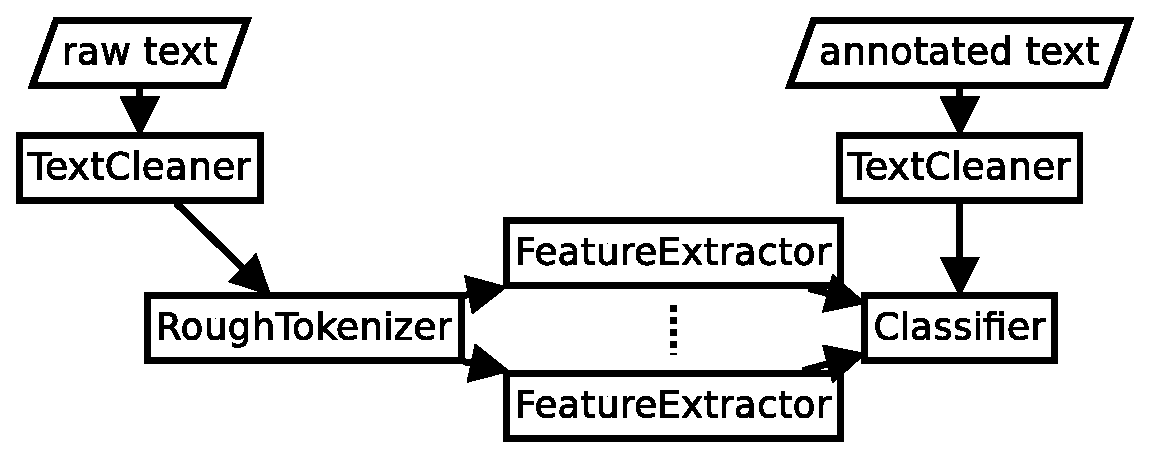
\includegraphics[width=\textwidth]{img/train-parts.eps}
  \caption{Data flow of the system in the training and evaluation
           configurations}
  \label{fig:train-parts}
\end{figure}

The Classifier is responsible for aligning the stream of rough tokens from the
input with the annotated text. The produced contextual information from the
tokens and the outcomes inferred from the aligned data are sent to the Maximum
Entropy Toolkit to serve as training data. After all the input files have been
processed and the training examples collected, the maximum entropy model is
computed and stored in a file for later use.

\subsection{Tokenization}

After a model has been trained, the tokenization mode becomes available. In
this mode the text is cleaned, converted into rough tokens and tagged with
properties. The Classifier has the trained model loaded and predicts the
outcome (sentence boundary, token boundary or no boundary) for every decision
point given its context. This outcome is used to resolve the \maysplit{},
\mayjoin{} and \maybreaksentence{} ambiguities and the disambiguation is stored
in the relevant rough token's metadata. These annotated tokens are then printed
through the OutputFormatter and encoded with the Encoder. See the setup of the
system in this mode on figure~\ref{fig:tokenize-parts}.

\begin{figure}
  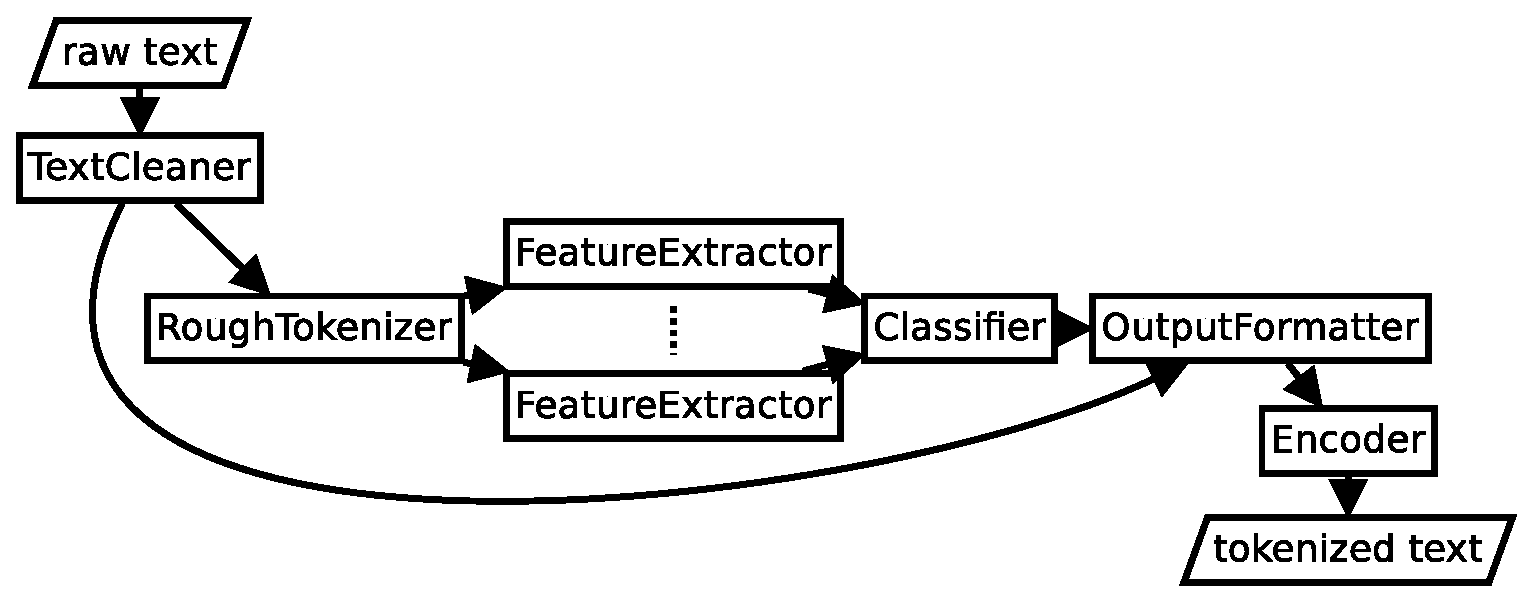
\includegraphics[width=\textwidth]{img/tokenize-parts.eps}
  \caption{Data flow of the system in the tokenization and preparation
           configurations}
  \label{fig:tokenize-parts}
\end{figure}

\subsection{Evaluation}

When tweaking and developing a tokenization system (the selected training data,
the configured parameters in the tokenization scheme) it is vital to have
feedback on the shortcomings of your system. The evaluation mode was designed
just for this purpose. It works in a way similar to the training mode (see
figure~\ref{fig:train-parts}). The Classifier aligns the rough tokens with the
annotated text and extracts the contextual properties from the tokens and the
true outcome from the annotated data. However, instead of recording them it
uses an already trained model and queries it for its predicted outcome. The
tokenizer then outputs both the true and the predicted outcome along with the
contextual properties.

Another tool can then be used to analyze the tokenizer's output and examine the
results and errors of the trained model. An example of such a tool would be the
included Python script analyze.py, which scans the evaluation's output and
reports the accuracy, precision, recall and F-measure of both sentence and
token boundary detection.

This log of outcomes and contexts can be written out when using any of the
available modes but only the evaluation mode has access to both the true
outcomes from the annotated data and the outcomes predicted by the
probabilistic model.

\subsection{Preparation}

The preparation is the last and least essential mode of the tokenizer. It is
similar to the tokenization mode (see figure~\ref{fig:tokenize-parts}), but
instead of querying the probabilistic model for an outcome, the Classifier
simply confirms all potential boundaries (\maysplit{} becomes a token boundary
and \maybreaksentence{} becomes a sentence boundary). This produces a file in
which an annotator only has to remove spaces and line breaks where
inappropriate to get the correct annotation.

An advantage to using this mode might be that when the user does not demand the
logging of contexts as in the evaluation mode, the time-costly FeatureExtractor
and Classifier can be replaced with a SimplePreparer, which only removes the
ambiguities in the abovementioned way.
